
%% INTRODUCTION %% 

\chapter{Introduction}


\section{The Bachelor's Thesis Problem}
People are becoming more interested in matters concerning physical and mental health. This is most likely attributed to the COVID-19 pandemic that has been circulating in recent years. Along with positive outcomes, such as increased care for fellow citizens and greater awareness of health issues, the consistent growth of interest in health issues also caused problems. With an increasing number of anxious and concerned patients, medical practices and general practitioners have long since exceeded their capacity limits and have reached their breaking point. This is also noticed by the patients: Overcrowded waiting rooms combined with long waiting periods and nerve-racking telephone loops are becoming the norm for doctor visits. The bachelor`s thesis problem can be traced back to the preceeding situation. The population is fearful, mainly caused by the COVID-19 pandemic, and doctors are reaching their limits. The resulting problems are of great importance. General practitioners are being forced to order patient stops and issue access bans. This also means that patients in need of immediate medical attention may be turned away and medical care may be denied. In addition to the concerned patients, the number of seriously (COVID-19) ill people has steadily increased: there have been approximately 146,000 deaths in Germany since the start of the pandemic (as of August 19, 2022). A survey was launched to highlight the problem in more detail (all questions included in the survey and the corresponding answers can be taken from the appendix). The results have shown that around 80\% of those questioned have put off a visit to the doctor in recent years, even though they have suffered from symptoms.
\begin{figure}[h]
	\centering
	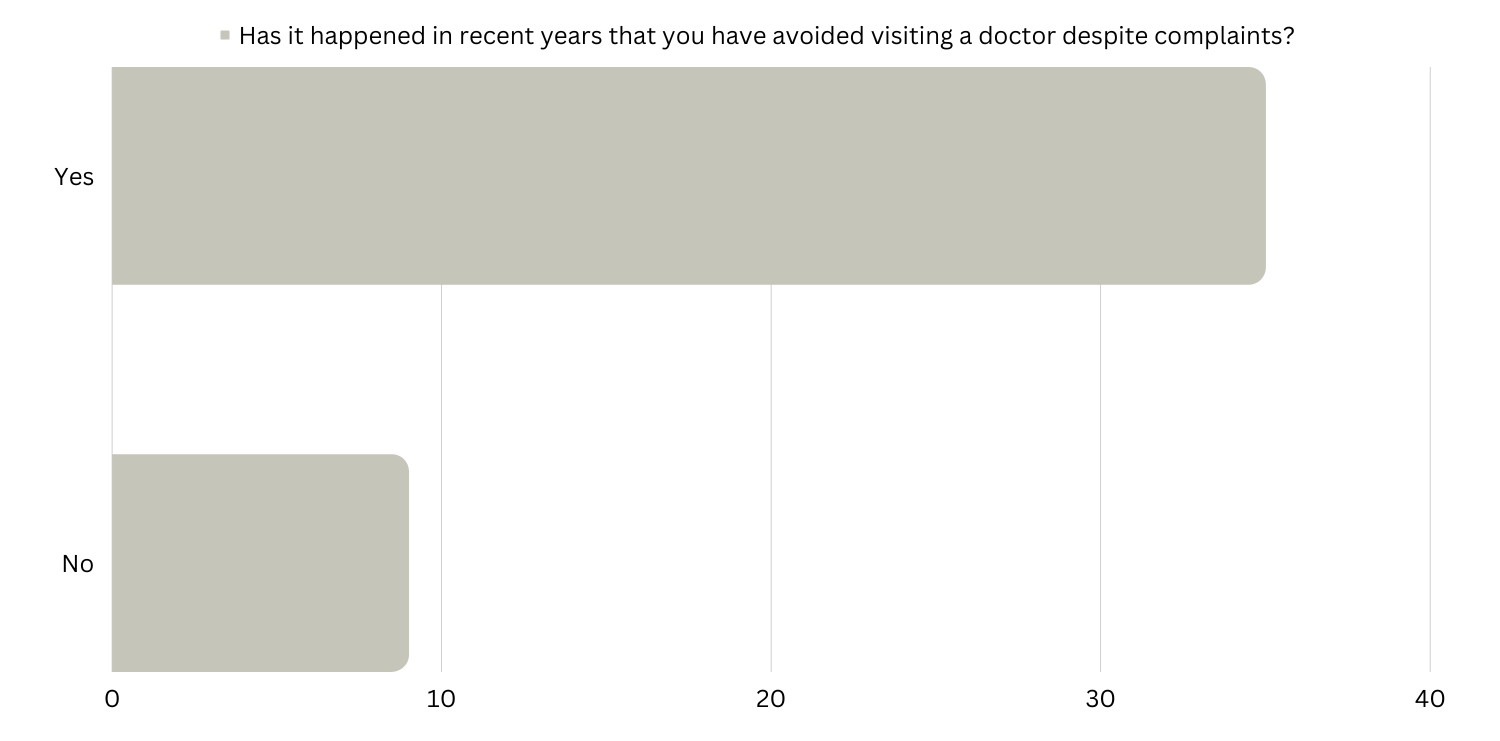
\includegraphics[scale=0.3]{question1.png}
	\caption[Survey Question]{Survey Question - Avoiding to visit the doctor}
\end{figure}

Another question within this survey was which reasons were the reason for postponing these doctor visits, or why the respondents could imagine avoiding a doctor visit. Those reasons range from long waiting times, to not being able to make an appointment. Figure 1.2 shows the mentioned distribution of the answers.
\begin{figure}[h]
	\centering
	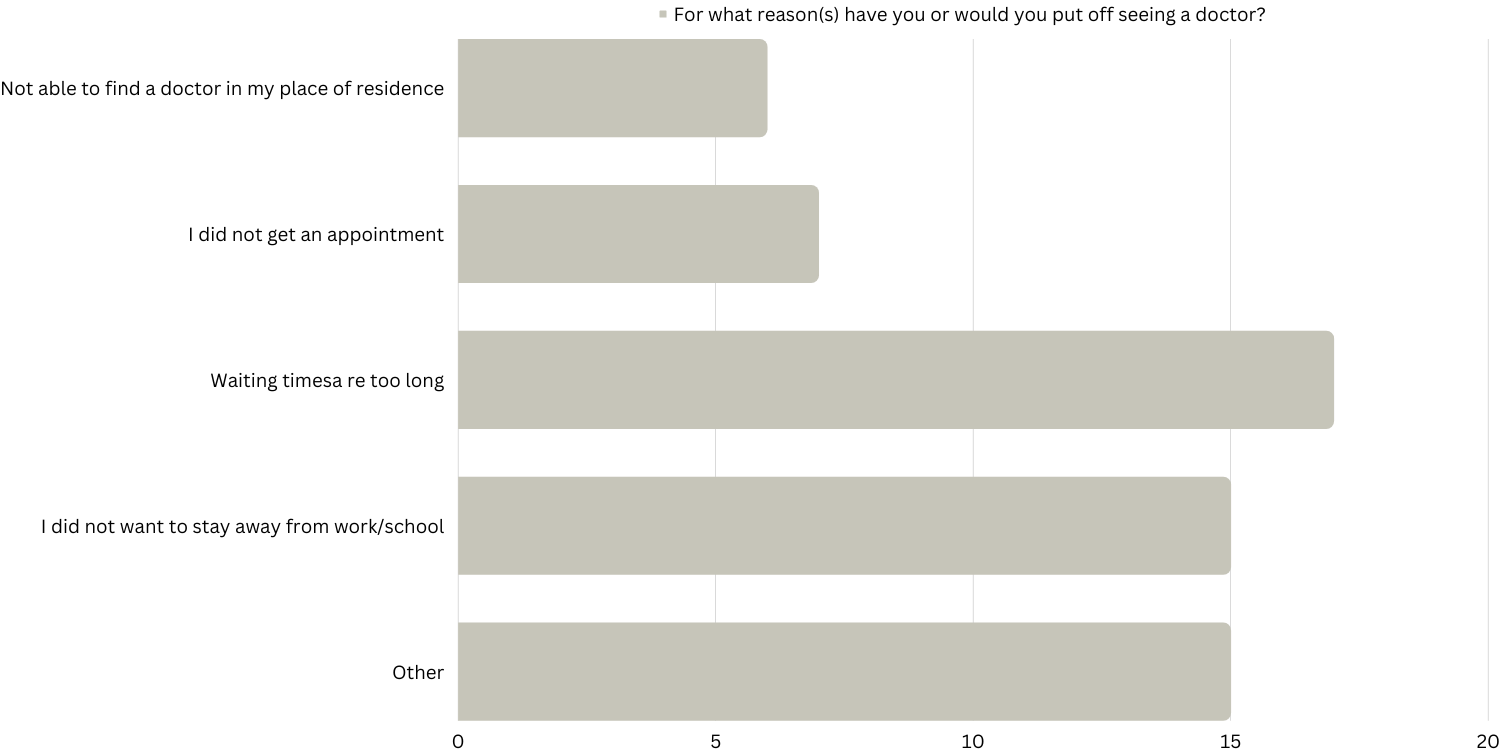
\includegraphics[scale=0.4]{question2.png}
	\caption[Survey Question]{Survey Question - Reasons of avoiding to visit the doctor}
\end{figure}

\section{Motivation}
The mentioned problem imposes the question on how to address patients’ concerns while also relieving the burden on doctors. Digitalization provides a solution to this problem. Online consultation hours and online appointment scheduling have recently helped relieve medical practices. Smartphones, in particular, are becoming an increasingly important part of our daily lives. The goal of this bachelor thesis is to provide a method for efficiently minimizing the aforementioned problems through the use of mobile applications. Such an application can provide advice to a worried user and help alleviate their fears.

\section{The Bachelor Thesis Goal}
The project's ultimate objective is the successful creation of a mobile application that enables users to receive a diagnosis based on the symptoms they reported, even if they were unable to schedule an appointment with a doctor, due to busy practices, or did not have the opportunity to see one, due to lack of time or long waiting times. This diagnosis is made after successful data gathering regarding the user's symptoms and a subsequent determination of the possible diseases. Another goal of the application is that the database can be expanded by doctors, whereby a verification possibility must be provided. They should be provided with the possibility to add either disease-related data or pieces of advice regarding diseases and illnesses for users. The detailed determination of how all of this should be made possible will be determined and implemented during the development process.